\subsection*{Additional MiniRocket reference on the fixed power18 input}
\label{sec:matched-p18}

To reduce the input-representation mismatch in the earlier comparison, we
added an official MiniRocket reference~\cite{dempster2021} on the same fixed
18-stream, 500-position log-mean-power input used by the spectral extension.
The reference retains the same participant roles, three outer folds, five
training seeds and test masks. Three previously fitted source configurations
were reused, and 12 further source fits completed the 15 fold/seed
configurations. These are 15 reference models, not 15 new datasets or an
additional selection among target scores. The source and evaluation freezes
and independent output checks bind the saved configurations and predictions.
No E weights were retrained for this comparison. The official multivariate MiniRocket transform uses 9,996 features (10,000 requested), maximum dilations per kernel 32, and separately reset NumPy and Numba random generators for each training seed. Transform parameters and a feature scaler with no centering are fitted only on the 504 source-training recordings; ridge regularization is fixed at $\alpha=1$. A scalar temperature in $[0.1,10]$ minimizes NLL only on the 168 clean source-validation recordings and is retained under loss.

The alignment is deliberately limited. E uses loss augmentation and
actual-mask features, whereas MiniRocket is clean-trained. At test time the
reference receives missing power18 entries filled with source-training band
means; it has no explicit mask or distance channel. The comparison therefore
aligns input representation and prediction roles, but not training policy,
loss treatment or classifier family. It is a useful additional reference,
not a controlled attribution of a difference to architecture or to support
matching. It was added after E's outcomes were known, so its status is
post-hoc and exploratory; it is not a new confirmation of the original
primary hypothesis or a state-of-the-art claim.

Table~\ref{tab:matched-p18} reports every complete, random-loss and
contiguous-loss condition for E, MiniRocket and the A/B hybrid controls,
including familiar-environment results. Metrics are calculated from saved
probabilities. For each training seed and loss-mask realization, held-fold
predictions are concatenated before calculating accuracy, seven-class macro
F1, NLL and summed multiclass Brier. Masks are then averaged within the
training seed; the displayed mean and sample SD are over five training
seeds. Complete input has one realization; each loss condition has five.
These SDs are not confidence intervals. The pooled familiar summary contains
504 fold-specific prediction occurrences, with possible repeat recordings
and participants across folds, rather than 504 independent new recordings.

\paragraph{Results and retained controls.}
E's pooled held accuracy is $75.175\pm1.005$\% on complete input, compared
with $53.841\pm0.938$\% for this MiniRocket reference. Under random 50\% loss,
the respective values are $73.822\pm0.942$\% and $22.305\pm1.102$\%;
under contiguous 50\% loss they are $60.597\pm1.375$\% and
$19.406\pm2.330$\%. Corresponding held macro F1 under contiguous loss is
$59.159\pm1.610$\% for E and $15.636\pm4.147$\% for the reference.
NLL is $1.160\pm0.014$ versus $4.852\pm1.764$, and Brier is
$0.552\pm0.011$ versus $1.275\pm0.168$, in that condition. This reference
degrades sharply under its declared mean-fill policy; the observation does
not establish that all MiniRocket training or repair configurations behave
similarly. Figure~\ref{fig:matched-p18} retains the full complete-to-loss
comparison on a common percentage scale.

The A/B hybrid controls remain weaker on complete held input than this
reference: their accuracies are $48.302\pm2.627$\% and
$48.048\pm2.559$\%, respectively. Thus the added reference does not reverse
the negative result for the main hybrid A. E also remains imperfect under
loss: its contiguous-loss macro F1 is below 60\%, and its pooled familiar
accuracy is $53.325\pm1.480$\% in that condition, compared with
$20.579\pm4.082$\% for MiniRocket. Familiar and held cohorts must not be
treated as an isolated causal room intervention.

\paragraph{Paired contrasts and conditional uncertainty.}
The additional E-minus-MiniRocket held macro-F1 contrast under contiguous
50\% loss is $+43.524\pm3.639$ percentage points across the five paired
training-seed differences, after mask averaging. All five seed differences
are positive. The reported 95\% conditional bootstrap range is
$[39.879,47.054]$ percentage points. For each of 10,000 paired bootstrap
draws (seed 20261028), ten participants are sampled with replacement from
the ten observed participants in each fixed environment. The same participant
multiplicities apply to both models, all five training seeds and all five
contiguous-loss masks. Weighted pooled confusion counts yield macro F1 for
each training-seed/mask cell, and the 25 cell contrasts are averaged.
This preserves pairing and repeated-view dependence. Environments, trained
models, training/mask seeds and the observed dataset remain fixed.
The range is descriptive and conditional: it does not represent uncertainty
over new rooms or training datasets and is not corrected for post-hoc
selection or multiple comparisons. No p-value or population-level
confirmation is inferred from its exclusion of zero.

The original A-minus-B primary comparison is kept separate. It remains
$+0.543\pm0.654$ macro-F1 percentage points under contiguous loss, with four
positive and one negative training-seed difference; its corresponding
descriptive conditional range is $[0.041,1.068]$ points. A--B changes
endpoint weighting, centering and covariance normalization even on complete
input. Both A and B share ideal full-effective-support congruence invariance,
and E's feature-only counterpart with B's denominator was not evaluated.
Consequently the large additional E--reference contrast does not isolate a
benefit caused by support matching, replace the small primary contrast, or
confirm its proposed mechanism. A training-policy-matched comparison and
independent data remain necessary for broader claims.

\begin{table*}[t]
\centering
\caption{Fixed-power-input comparison, retaining E, the clean-trained MiniRocket reference (MR-P18), and both hybrid controls. C: complete; R50/B50: random/contiguous 50\% loss. Values are mean $\pm$ sample SD across five training seeds after mask averaging, not confidence intervals. Accuracy and macro F1 are percentages; NLL and summed multiclass Brier are unitless. Held pools 1,260 recordings; familiar pools 504 fold-specific prediction occurrences, with possible repeated recordings/participants across folds. E is loss-augmented; MR-P18 is clean-trained with source-band-mean fill and no mask input, so this is not a training-policy-matched architectural comparison.}
\label{tab:matched-p18}
\begingroup\fontsize{9.5}{12}\selectfont
\setlength{\tabcolsep}{4pt}\renewcommand{\arraystretch}{1.13}
\setlength{\extrarowheight}{1.3pt}\setlength{\arrayrulewidth}{0.5pt}\arrayrulecolor{mrefBorder}
\begin{tabularx}{\textwidth}{|lll*{4}{>{\raggedleft\arraybackslash}X}|}
\hline\rowcolor{mrefHead}
\mrefHeadText{Model} & \mrefHeadText{Cohort} & \mrefHeadText{Input} & \mrefHeadText{Accuracy (\%)} & \mrefHeadText{Macro F1 (\%)} & \mrefHeadText{NLL} & \mrefHeadText{Brier} \\
\hline
\rowcolor{mrefE}
E & Held & C & 75.17\,\(\pm\)\,1.00 & 74.61\,\(\pm\)\,1.21 & 0.773\,\(\pm\)\,0.018 & 0.365\,\(\pm\)\,0.008 \\
\rowcolor{mrefE}
E & Held & R50 & 73.82\,\(\pm\)\,0.94 & 73.33\,\(\pm\)\,1.10 & 0.831\,\(\pm\)\,0.018 & 0.386\,\(\pm\)\,0.009 \\
\rowcolor{mrefE}
E & Held & B50 & 60.60\,\(\pm\)\,1.37 & 59.16\,\(\pm\)\,1.61 & 1.160\,\(\pm\)\,0.014 & 0.552\,\(\pm\)\,0.011 \\
\rowcolor{mrefE}
E & Familiar & C & 68.41\,\(\pm\)\,1.26 & 67.97\,\(\pm\)\,1.39 & 0.883\,\(\pm\)\,0.051 & 0.448\,\(\pm\)\,0.019 \\
\rowcolor{mrefE}
E & Familiar & R50 & 66.40\,\(\pm\)\,0.84 & 65.77\,\(\pm\)\,0.93 & 0.946\,\(\pm\)\,0.051 & 0.470\,\(\pm\)\,0.014 \\
\rowcolor{mrefE}
E & Familiar & B50 & 53.33\,\(\pm\)\,1.48 & 51.51\,\(\pm\)\,1.64 & 1.341\,\(\pm\)\,0.059 & 0.648\,\(\pm\)\,0.019 \\
\hline
\rowcolor{mrefMR}
MR-P18 & Held & C & 53.84\,\(\pm\)\,0.94 & 53.87\,\(\pm\)\,1.01 & 1.363\,\(\pm\)\,0.037 & 0.634\,\(\pm\)\,0.009 \\
\rowcolor{mrefMR}
MR-P18 & Held & R50 & 22.30\,\(\pm\)\,1.10 & 16.11\,\(\pm\)\,0.84 & 3.486\,\(\pm\)\,0.151 & 1.109\,\(\pm\)\,0.023 \\
\rowcolor{mrefMR}
MR-P18 & Held & B50 & 19.41\,\(\pm\)\,2.33 & 15.64\,\(\pm\)\,4.15 & 4.852\,\(\pm\)\,1.764 & 1.275\,\(\pm\)\,0.168 \\
\rowcolor{mrefMR}
MR-P18 & Familiar & C & 58.85\,\(\pm\)\,0.57 & 58.30\,\(\pm\)\,0.77 & 1.295\,\(\pm\)\,0.043 & 0.588\,\(\pm\)\,0.010 \\
\rowcolor{mrefMR}
MR-P18 & Familiar & R50 & 22.38\,\(\pm\)\,1.37 & 15.84\,\(\pm\)\,1.40 & 3.388\,\(\pm\)\,0.282 & 1.105\,\(\pm\)\,0.043 \\
\rowcolor{mrefMR}
MR-P18 & Familiar & B50 & 20.58\,\(\pm\)\,4.08 & 16.75\,\(\pm\)\,5.85 & 4.812\,\(\pm\)\,1.797 & 1.263\,\(\pm\)\,0.194 \\
\hline
\rowcolor{mrefA}
A & Held & C & 48.30\,\(\pm\)\,2.63 & 47.55\,\(\pm\)\,2.93 & 1.395\,\(\pm\)\,0.052 & 0.690\,\(\pm\)\,0.028 \\
\rowcolor{mrefA}
A & Held & R50 & 49.58\,\(\pm\)\,1.76 & 49.15\,\(\pm\)\,1.99 & 1.327\,\(\pm\)\,0.032 & 0.665\,\(\pm\)\,0.024 \\
\rowcolor{mrefA}
A & Held & B50 & 34.77\,\(\pm\)\,1.37 & 34.04\,\(\pm\)\,1.38 & 2.127\,\(\pm\)\,0.084 & 0.902\,\(\pm\)\,0.021 \\
\rowcolor{mrefA}
A & Familiar & C & 49.76\,\(\pm\)\,1.86 & 48.59\,\(\pm\)\,1.62 & 1.402\,\(\pm\)\,0.061 & 0.677\,\(\pm\)\,0.020 \\
\rowcolor{mrefA}
A & Familiar & R50 & 49.33\,\(\pm\)\,0.45 & 48.39\,\(\pm\)\,0.48 & 1.352\,\(\pm\)\,0.029 & 0.660\,\(\pm\)\,0.009 \\
\rowcolor{mrefA}
A & Familiar & B50 & 40.16\,\(\pm\)\,1.30 & 39.46\,\(\pm\)\,1.05 & 1.904\,\(\pm\)\,0.072 & 0.822\,\(\pm\)\,0.012 \\
\hline
\rowcolor{mrefB}
B & Held & C & 48.05\,\(\pm\)\,2.56 & 47.24\,\(\pm\)\,2.78 & 1.412\,\(\pm\)\,0.046 & 0.696\,\(\pm\)\,0.029 \\
\rowcolor{mrefB}
B & Held & R50 & 49.23\,\(\pm\)\,1.89 & 48.48\,\(\pm\)\,2.19 & 1.361\,\(\pm\)\,0.040 & 0.673\,\(\pm\)\,0.029 \\
\rowcolor{mrefB}
B & Held & B50 & 34.19\,\(\pm\)\,1.60 & 33.49\,\(\pm\)\,1.56 & 2.143\,\(\pm\)\,0.083 & 0.908\,\(\pm\)\,0.021 \\
\rowcolor{mrefB}
B & Familiar & C & 49.68\,\(\pm\)\,1.36 & 48.67\,\(\pm\)\,1.11 & 1.413\,\(\pm\)\,0.056 & 0.681\,\(\pm\)\,0.016 \\
\rowcolor{mrefB}
B & Familiar & R50 & 48.98\,\(\pm\)\,0.87 & 48.08\,\(\pm\)\,0.26 & 1.364\,\(\pm\)\,0.030 & 0.665\,\(\pm\)\,0.008 \\
\rowcolor{mrefB}
B & Familiar & B50 & 39.73\,\(\pm\)\,1.35 & 39.31\,\(\pm\)\,0.96 & 1.930\,\(\pm\)\,0.060 & 0.831\,\(\pm\)\,0.015 \\
\hline
\end{tabularx}
\arrayrulecolor{black}\endgroup
\end{table*}

\begin{figure*}[t]
\centering
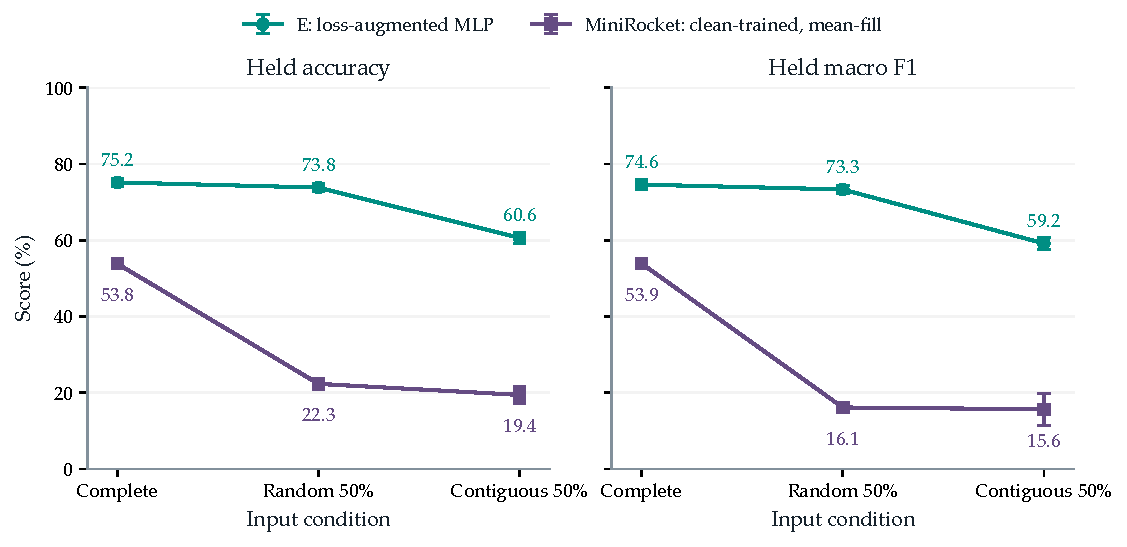
\includegraphics[width=.98\textwidth]{matched_power18_comparison.pdf}
\caption{Post-hoc comparison on the same fixed power18 representation and held prediction roles. Error bars are sample SD over five training seeds after within-seed mask averaging. The E--reference difference includes training and loss-treatment differences: E uses loss augmentation and actual-mask features; MiniRocket is clean-trained and receives source-band-mean-filled input without a mask. These curves do not isolate an architectural or support-matching effect and are not an independent confirmation or a state-of-the-art ranking. A/B controls and familiar results remain in Table~\ref{tab:matched-p18}.}
\label{fig:matched-p18}
\end{figure*}

